\documentclass[11pt,letterpaper]{article}
\input{../../preamble}
\usepackage{fullpage}
\usepackage{multicol}

\begin{document}
\flushleft
\begin{multicols}{2}

\begin{large}\textbf{Math 2554 Exam  2: Derivatives \\
date}\end{large}

\hfill\textbf{Name:  }\underline{\hspace{40ex}} %KEY\hspace{17ex}}

\vspace{.5in}

\end{multicols}

\pagestyle{empty}

\flushleft

\begin{enumerate}[I.]
% % % % % % % % % %
\item  \textbf{Definitions/Concepts.} 
	\begin{enumerate}[1.]
	% % %
	\item (3.2) Differentiate $\displaystyle y=\frac{x-a}{\sqrt{x}-\sqrt{a}}$ with respect to $x$, using any method you like.
	
	% % %
	\item (3.3) Use the Quotient Rule to find $\displaystyle\dfrac{d}{dx}\left(\frac{1}{x^n}\right)$.  In this problem, $n$ is a positive integer.
	
	% %%
	\item {\bf ChAlLeNgE or Extra Credit} (3.4) Using the trig identity 
	\[\sin{2x}=2\sin x\cos x\]
	find $\displaystyle\dfrac{d}{dx}\left(\sin{2x}\right)$.
		
	% % %
	\item {\bf ChAlLeNgE} (3.4) Use the trig identity
	\[\cos^2x+\sin^2x=1\] 
	to prove that 
	\[\lim_{x\to 0}\frac{\cos x-1}{x}=0.\]

	% % %
	\item (3.5) Suppose a company produces $x$ items at a cost $C(x)$.
		\begin{enumerate}[(a)]
		\item Write a formula for the {\bf average cost}.
		\item Write a formula for the {\bf marginal cost}.
		\item Suppose $\Delta x=1$ item.  In words, what is $\displaystyle\frac{\Delta C}{\Delta x}$?
		\end{enumerate}
		
	% % %
	\item (3.6) Suppose $f(x)$ and $g(x)$ are differentiable at all values of $x$.  Then 
	\[f(g(x^2))=\]	
	
	\end{enumerate}
	
% % % % % % % % % %
\vspace{1pc}
\item \textbf{Questions/Problems.} 
	\begin{enumerate}[1.]
	% % % 
	\item (3.2) $f(x)=2x^3-3x^2-12x+4$
		\begin{enumerate}[(a)]
		\item Find all points on the graph of $f$ at which the tangent line is horizontal.
		\item Find all points on the graph of $f$ at which the tangent line has slope 60.
		\end{enumerate}
		
	% % %
	\item (3.2) Let $F=f+g$ and $G=3f-g$, where the graphs of $f$ and $g$ are shown in Figure \ref{fig:graphDeriv}.
	
	\vspace{-0.5pc}  
	\begin{figure}[h]
	\begin{center}
	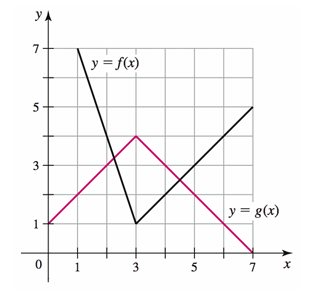
\includegraphics[scale=0.8]{Exam2graphDeriv.png}
	\caption{(Briggs, W. and Cochran, L. \emph{Calculus: Early ranscendentals})}
	\label{fig:graphDeriv}
	\end{center}
	\end{figure}
	
	Find the following derivatives:
		\begin{enumerate}[(a)]
		\item $F'(1)$
		\item $G'(1)$
		\item $F'(5)$
		\item $G'(5)$
		\end{enumerate}
		
	% % %
	\item (3.3) Let $f(t)=100e^{-0.05t}$.
		\begin{enumerate}[(a)]
		\item Find the values of $t$ for which the slope of the curve $y=f(t)$ is $-5$.
		\item Does the graph of $f$ have a horizontal tangent line?
		\end{enumerate}
	
	% % %	
	\item (3.4) For what values of $x$ does $f(x)=x-\cos x$ have a horizontal tangent line?
		
	% % %
	\item (3.5) Suppose a stone is thrown vertically upward from the edge of a cliff on mars (where the acceleration of gravity is only about 12 ft/s\textsuperscript{2}) with an initial velocity of 64 ft/s from a height of 192 ft above the ground.  The height $s$ of the stone above the ground after $t$ seconds is given by 
	\[s=-6t^2+64t+192.\]
		\begin{enumerate}[(a)]
		\item Determine the velocity $v$ of the stone after $t$ seconds.
		\item When does the stone reach its highest  point?
		\item What is the height of the stone at the highest point?
		\item When does the stone strike the ground?
		\item With what velocity does the stone strike the ground?
		\end{enumerate}
	
	% % %
	\item (3.7) For each function $(g(x)$, find the value of $g'(3)$ using the data given below.
	\begin{align*}
	f(1)=6 & \qquad f(3)=2 & f(6)=5 & \qquad f(9)=-3\\
	f'(1)=-2 & \qquad f'(3)=4 & f'(6)=-1 & \qquad f'(9)=1
	\end{align*}
		\begin{enumerate}[(a)]
		\item $g(x)=f(3)+10f(2x)$
		\item $g(x)=\displaystyle\frac{f(x^2)}{x}$
		\item $g(x)=\left(f(x)\right)^3$
		\item $g(x)=f(\sqrt{2}\sin{\frac{\pi}{4}x})$                                        
		\end{enumerate}
		
	\end{enumerate}	
% % % % % % % % % %
\vspace{1pc}
\item \textbf{Computations/Algebra.} 
	\begin{enumerate}[1.]
	% % %
	\item (3.2) $f(x)=3x^2+5e^x$
	
	Find $f'(x),\,f''(x),$ and $f^{(3)}(x)$.
	
	% % %
	\item (3.2) Find the derivative of $h(x)=(x^2+1)^2$.
	
	% % %
	\item (3.2) Find the derivative of $h(x)=\sqrt{x}\left(\sqrt{x}-1\right)$.
	
	% % %
	\item (3.2) Find the derivative of the following functions:
		\begin{enumerate}[(a)]
		\item $y=x^5$
		\item $f(v)=v^{100}$
		\item $8x$
		\item $g(w)=2w^3+3w+e^w$
		\end{enumerate}
		
	% % %
	\item (3.3) Find the derivative of the following functions:
		\begin{enumerate}[(a)]
		\item $\displaystyle h(x)=\frac{(x-1)(2x^2-1)}{x^3-1}$
		\item $\displaystyle h(x)=\frac{x+1}{x^2e^x}$
		\end{enumerate}
		
	% % %
	\item (3.4) Evaulate the following limits:
		\begin{enumerate}[(a)]
		\item $\displaystyle\lim_{x\to 0}\frac{\sin{3x}}{x}$
		\item $\displaystyle\lim_{x\to 0}\frac{\tan{5x}}{x}$
		\item $\displaystyle\lim_{x\to -3}\frac{\sin{(x+3)}}{x^2+8x+15}$
		\end{enumerate}
	
	% % %	
	\item (3.4) Find $y'$ for each of the following functions:
		\begin{enumerate}[(a)]
		\item $y=\sin x+\cos x$
		\item $y=5x^2+\cos x$
		\item $\displaystyle y=\frac{(x^2-1)\sin x}{\sin x+1}$
		\end{enumerate}
	
	% % %
	\item (3.6) $y=x\cos{x^2}$
	
	Find $\displaystyle\dfrac{d^2y}{dx^2}$.
	
	% % %
	\item (3.6) Find the derivative of $f(x)=(\cos x+2\sin x)^8$.
	
	% % %
	\item (3.6) Find the derivative of $f(x)=\sin^5{(\cos{3x})}$.
	
	% % %
	\item (3.7) Find $\displaystyle\dfrac{dy}{dx}$.
		\begin{enumerate}[(a)]
		\item $\sin{(xy)}=x+y$
		\item $e^{xy}=2y$
		\item $(xy+1)^3=x-y^2+8$
		\end{enumerate}
		
	% % %
	\item (3.7) For each function find $\displaystyle\dfrac{d^2y}{dx^2}$.
		\begin{enumerate}[(a)]
		\item $x^4+y^4=64$
		\item $e^{2y}+x=y$
		\end{enumerate}
	
	\end{enumerate}

% % % % % % % % % %	
\end{enumerate}
\end{document}


